\documentclass{article}

\usepackage[english]{babel}
\usepackage[utf8]{inputenc}
\usepackage{fancyhdr}
\usepackage{amsmath}
\usepackage{amssymb}
\usepackage{setspace} 
\usepackage{graphicx}
\usepackage{float}
\usepackage{tabularx}

\usepackage{chngpage}



\pagestyle{fancy}
\fancyhf{}
\lhead{MSE160: Formula sheet/Notes}
\rhead{Youssef El Mays}
\doublespacing



\newcommand{\SubItem}[1]{
    {\setlength\itemindent{15pt} \item[-] #1}
}

\newcolumntype{L}{>{\centering\arraybackslash}m{3cm}}

\textheight = 650pt


\begin{document}
    \title{MSE160: Formula Sheet/Notes}
    % \begin{titlepage}
    %     \tableofcontents
    % \end{titlepage}
    

    \section{Atomic Structure}
    \subsection{Energy}
    \begin{flalign}
        &u_vdv = \frac{8\pi v^2}{c^3} \cdot \frac{hv}{e^{\frac{hv}{K_bT}}-1} &\\
        &E=hv
    \end{flalign}
    \subsection{Photoelectric Effect}
    \begin{flalign}
        &\frac{1}{2}m_ev^2_k = E_k = hv - W&\\
        &\frac{1}{\lambda} = R_H\left( \frac{1}{n_1^2} -  \frac{1}{n_2^2}\right) \\
        & R_H = 1.097373\times 10^7m^{-1}\\
        & n_1 = 1 \Rightarrow Lyman \\
        & n_1 = 2 \Rightarrow Balmer \\
        & n_1 = 3 \Rightarrow Paschen \\
        & n_1 = 4 \Rightarrow Brackett \\
        & n_1 = 5 \Rightarrow Pfund \\
        & n_2 > n_1
    \end{flalign}
    \subsection{De Broglie Relationship}
    \begin{flalign}
        & E^2 = p^2c^2 + m^2c^4 &\\
        & \text{for zero rest mass: } E^2 = p^2c^2 \rightarrow E = pc \\
        & hv = h\frac{c}{\lambda} = pc \\
        & \therefore p = \frac{h}{\lambda}
    \end{flalign}
    \subsection{Electron diffraction}
    \begin{flalign}
        & E_K = eV - \frac{p^2}{2m}& \\
        & p = \sqrt{2meV} \\
        & \lambda = \frac{h}{\sqrt{2meV}} \\
        & \lambda = 2d\sin(\theta) \\
        & \sin^2(\theta) = \frac{C}{V},\;\text{Where }C=\frac{h^2}{8med^2}
    \end{flalign}
    \subsection{Bohr Model}
    \begin{flalign}
        & F_{centripedal} = F_{electric} &\\
        & m\frac{v^2}{r} = \frac{e^2}{4\pi \epsilon_0 r^2} \\
        & \therefore v^2 = \frac{e^2}{4\pi\epsilon_0 mr} \\ 
        & I_{orbit} = n\lambda = 2\pi r \;\text{Where n is the quantisation condition} \\
        & \therefore v = \frac{hn}{2 \pi m r} \\
        & L = mvr = n\frac{h}{2\pi} = n \hbar \\ 
        & \text{As such, allowed radii are described by the expression:} \\
        & r_n = \frac{h^2\epsilon_0n^2}{\pi me^2} = a_{Bohr} n^2 \\ 
        & r_1 = a_{Bohr} = \frac{h^2\epsilon_0}{\pi me^2} = 5.3\times 10^{-11}m \\
        & E_k = \frac{1}{2}mv^2 = \frac{e^2}{8\pi \epsilon_0 r} \\
        & E_T = E_k + E_c = \frac{e^2}{8\pi \epsilon_0 r} - \frac{e^2}{4\pi \epsilon_0 r^2} = - \frac{e^2}{8\pi \epsilon_0 r} \\
        & \text{Substiting in $r_n$ gives:} \\
        & E_T = -\left(\frac{me^4}{8\epsilon_0^2h^2}\right)\cdot \frac{1}{n^2} = \frac{-13.6eV}{n^2},\;1\;eV \approx 1.602\times 10^{-19}J \\
        & \Delta E = E_i - E_f = \frac{me^4}{8\epsilon_0^2h^2}(\frac{1}{n^2_f} - \frac{1}{n^2_i}) \\
        & \text{since: }\;E=hv=h\frac{c}{\lambda} \\
        & \frac{1}{\lambda} = \frac{me^4}{8\epsilon_0^2h^3}\left(\frac{1}{n^2_f} - \frac{1}{n^2_i}\right) = R_H\left(\frac{1}{n^2_f} - \frac{1}{n^2_i}\right)
    \end{flalign}
    \subsection{Waves}
    \begin{flalign}
        & \Psi = Ae^{i(kx - \omega t)} &\\
        & k = 2\pi/\lambda \\
        & \omega=2\pi v \\ 
        & c = v\lambda = \frac{\omega}{2\pi}\cdot \lambda = \frac{\omega}{\lambda} \\
        & P(x) \propto |\Psi|^2dx \\
        & \frac{\partial\Psi}{\partial x} = ikAe^{i(kx - \omega t)} = ik\Psi \\
        & \frac{\partial\Psi}{\partial t} = -i\omega Ae^{i(kx - \omega t)} = i\omega\Psi \\
        & \text{De Broglie: } p = \frac{h}{\lambda} = \frac{h}{2\pi}\cdot\frac{2\pi}{\lambda} = \hbar k \\
        & \text{Enstein: } E = hv = h \frac{\omega}{2\pi} = \hbar\omega \\
        & \frac{\partial}{\partial x} \Psi = i \frac{p}{\hbar}\Psi \Rightarrow p\Psi = \{-i\hbar\frac{\partial}{\partial x}\}\Psi\\
        & \frac{\partial}{\partial t} \Psi = -i \frac{E}{\hbar}\Psi \Rightarrow E\Psi = \{i\hbar\frac{\partial}{\partial t}\}\Psi \\
        & \Delta t = \frac{1}{\Delta f} = \frac{h}{\Delta E} \Rightarrow \Delta E \cdot \Delta t \geq h \\
        & \Delta x = \Delta \lambda_{dB}= \frac{h}{\Delta p} \Rightarrow \Delta x \cdot \Delta p \geq h
    \end{flalign}
    \textbf{Heisenber's Uncertainty Principle:}\\
    It is impossible to specify simultaneously, with precision, both the momentum and the position of a particle.
    \subsection{Shrodinger's Equation Derivation}
    \begin{flalign}
        & E = E_k + E_p = \frac{1}{2}mv^2 + V = \frac{p^2}{2m} + V &\\
        & i\hbar\frac{\partial}{\partial t}\Psi(x,t) = -\frac{\hbar^2}{2m}\frac{\partial^2}{\partial x^2}\Psi(x,t)+V\Psi(x,t)
    \end{flalign}
    \subsection{Time independent Shrodinger's Equation}
    \begin{flalign}
        & \Psi(x,t) = \phi(t)\psi(t) &\\
        & i\hbar\frac{1}{\phi(t)}\frac{\partial\phi(t)}{\partial t} = -\frac{\hbar^2}{2m\psi(x)}\frac{\partial^2\psi(x)}{\partial x^2}+V \\
        & \therefore \; i\frac{A}{\hbar}\phi=\frac{\partial\phi(t)}{\partial t} \\
        & \phi(t) = Ce^{-i(\frac{A}{\hbar})t} \Rightarrow \frac{d \phi(t)}{d t} = -i(\frac{A}{\hbar})Ce^{-i(\frac{A}{\hbar})t}\\
        & \text{By unit analysis: } A=E \\
        & \therefore \; E\psi=-\frac{\hbar^2}{2m}\frac{d^2\psi}{d x^2} + V\psi
    \end{flalign}
    \subsection{Electron in a box}
    \begin{flalign}
        &V(0) = V(L) = \inf& \\
        & V(x) = 0\; \forall\, x \,|\, 0<x<L \\
        & \therefore\, -\frac{\hbar^2}{2m}\frac{d^2\psi}{d x^2} = E\psi \\
        & \text{General Solution: } \psi = A\sin(kx) + B\cos(kx) \\
        & \frac{d^2\psi}{dx^2} = -k^2(A\sin(kx)) + B\cos(kx)) = -k^2\psi \\
        & -\frac{\hbar^2}{2m}\frac{d^2\psi}{d x^2} = \left(-\frac{\hbar^2}{2m}\right) \cdot (-k^2\psi) = E\psi \\
        & E = \frac{\hbar^2k^2}{2m} \\
        & \text{Applying boundary conditions: } \\
        & \psi(0) = 0 \Rightarrow B = 0 \\
        & \psi(L) = 0 \Rightarrow A=0 \;or\;\sin(kL)=0 \\
        & \therefore kL=n\pi,\; n=1,2,3... \\
        & \psi_n = A\sin(\frac{n\pi x}{L}) \\
        & E_n = \frac{h^2}{8mL^2}\cdot n^2 \\
        & 1 = \int_0^L A^2\sin^2(\frac{n\pi x}{L})dx \Rightarrow A = \sqrt{\frac{2}{L}} \\
        & \psi_n =\sqrt{\frac{2}{L}} \sin(\frac{n\pi x}{L}) \\
        & P_n(x) = \frac{2}{L}\sin^2(\frac{n\pi x}{L})dx
    \end{flalign}
    \subsection{3D}
    \begin{flalign}
        & -\frac{\hbar^2}{2m} \left(\frac{d^2}{d x^2} + \frac{d^2}{d y^2} + \frac{d^2}{d z^2}\right) \psi + V\psi = E\psi & \\ 
        & \nabla = \left(\frac{d}{d x} + \frac{d}{d y} + \frac{d}{d z}\right) \\ 
        & -\frac{\hbar^2}{2m}\nabla^2\psi + V\psi = E\psi
    \end{flalign}
        There are 3 spacial degrees of freedom and 1 spin degree of freedom, therefore there are 4 quantum numbers \\
        n = Principle quantum numbers, $\{n\,|\, n \in \mathbb{N}\} $ \\
        $\ell$ = Orbital quantum number $\{\ell\,|\,0\leq \ell \leq n - 1,\; \ell \in \mathbb{W} \}$ \\
        $m_\ell$ = Magnetic quantum number $\{m_\ell\,|\,-\ell \leq m_\ell \leq \ell,\;m_\ell\in\mathbb{Z}\} $\\
        $m_s$ = Spin quantum number $\{ m_s\,|\, m_s \in \{\frac{1}{2},\,-\frac{1}{2}\} \}$

    \section{Bonding and Crystaline Structure}
    \begin{table}[H]
        \begin{adjustwidth}{-.8in}{-.8in}  
        \centering
        \begin{tabularx}{1.3\textwidth}{| c | L | L | L | >{\centering\arraybackslash}X |}
            \hline
            \textbf{Bond} &
            \textbf{Action with Charges}&
            $\mathbf{\varDelta E}$& 
            $\mathbf{E_{avg}}$ &
            \textbf{Bond Energy}\\
            \hline
            \textbf{Ionic} &
            Exchange &
            High&
            Low &
            Large \\
            \hline
            \textbf{Covalent} &
            Sharing &
            Low&
            High &
            Variable \\
            \hline
            \textbf{Metalic} &
            Delocalized Sharing &
            Low &
            Low & 
            Variable\\
            \hline
        \end{tabularx}
    \end{adjustwidth}
    \end{table}
    \subsection{I don't have a good title yet}
    \begin{flalign}
        &E_N = E_A+E_R = -\frac{A}{r} + \frac{B}{r^n} &\\
        & ionic\;character = 1-e^{-\frac{(X_A - X_B)^2}{4}} \\
        &\frac{\varDelta L}{L_0} = \alpha\left(T_2-T_1\right) \\
        & APF = \frac{n_a \cdot \frac{4}{3}\pi r_a^3 }{a^3}
    \end{flalign}
    \begin{table}[H]
        \begin{adjustwidth}{-.4in}{-.4in}  
            \centering
            \begin{tabularx}{1.1\textwidth}{| X | L | L | c |}
                \hline
                \textbf{Structure} & 
                \textbf{Coordination Number} & 
                \textbf{Atoms/unit cell} &
                \textbf{APF} \\
                \hline
                Simple Cubic &
                6 &
                8 &
                0.52 \\
                \hline
                Body Centered Cubic (BCC) &
                8 &
                2 &
                0.68 \\
                \hline
                Face Centered Cubic &
                12 &
                4 &
                0.74\\
                \hline
            \end{tabularx}
        \end{adjustwidth}
    \end{table}

    \subsection{Some densities}
    \begin{flalign}
        & \rho = \frac{nA}{V_cN_a} & \\
        &LD = \frac{n_a}{r} \\
        & PD = \frac{n}{a^2}
    \end{flalign}

    \subsection{X-Ray Diffraction} 
    \begin{flalign}
        & d = \frac{n\lambda}{2\sin(\theta_c)} & \\
        & d = \frac{a}{\sqrt{i^2+j^2+k^2}}
    \end{flalign}
    d = planar spacing \\
    $\theta_c$ = critical angle

    \subsection{Imperfections and Diffusion}
    \subsubsection{Solidification}
        \textbf{Nucleation:} Nuclei of solid form in liquid \\
        \textbf{Growth:} Nuclei grow to form crystals – crystals grow until all liquid consumed leaving grains  
    \begin{figure}[H]
        \centering
        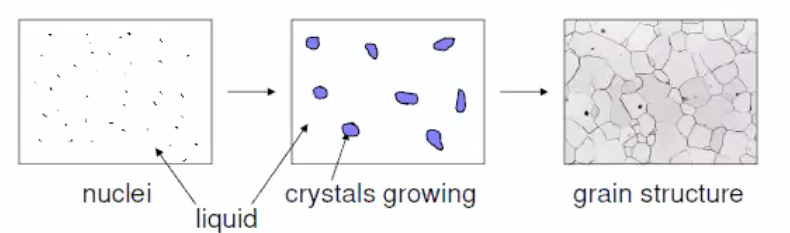
\includegraphics[width=\textwidth]{images/solidification.png}
    \end{figure}
    \textbf{Grain types:}
    \begin{enumerate}
        \item Equiaxed: Same size in all directions
        \item Columnar: Elongated
    \end{enumerate}

    \subsubsection{Imperfections}
    \textbf{Types of Imperfections:}
    \begin{enumerate}
        \item Point Defects
            \SubItem{Vacancies} 
            \SubItem{Interstitial Atoms}
            \SubItem{Substitutional Atoms}
        \item Line Defects
            \SubItem{Dislocations}
        \item Areal Defects
            \SubItem{Grain boundaries}
    \end{enumerate}

    \textbf{Vacancy:}
    \begin{figure}[H]
        \centering
        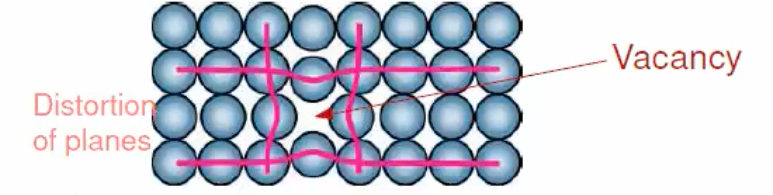
\includegraphics[width=\textwidth]{images/vacancy.png}
    \end{figure}
    \textbf{Interstitial Atoms}
    \begin{figure}[H]
        \centering
        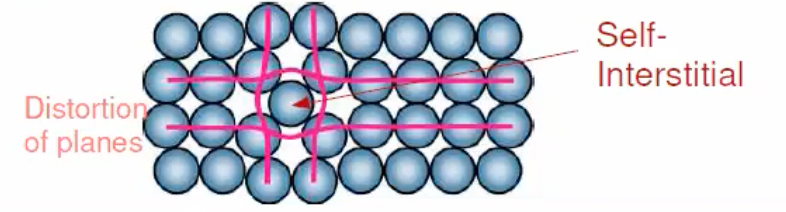
\includegraphics[width=\textwidth]{images/Interstitial.png}
    \end{figure}

    \begin{flalign}
       & \frac{N_v}{N} = e^{\frac{-Q_v}{kT}} & \\
       & k = 1.38\times 10^{-23} \frac{J}{atom \cdot K} = 8.62 \times 10^{-5}\frac{eV}{atom \cdot K}  \\
       & N = \rho V \frac{N_A}{A}
    \end{flalign}
    $N_v$ = No. of Defects \\
    $N$ = No. of potential defect sites \\
    $Q_v$ = Activation Energy\\\\
    \textbf{Conditions for substitutional solid solutions: Hume – Rothery rules}
    \begin{enumerate}
        \item $\varDelta r < 15\%$
        \item Proximity in periodic table (Low $\varDelta E$)
        \item Same crystal structure for pure metals
        \item Valency
    \end{enumerate}
    \textbf{Edge Dislocations}
    \begin{enumerate}
        \item Extra half plane inserted into a crystal structure
        \item Burgers Vector, b is perpendicular $\perp$ to the dislocation line
    \end{enumerate}
    \begin{figure}[H]
        \centering
        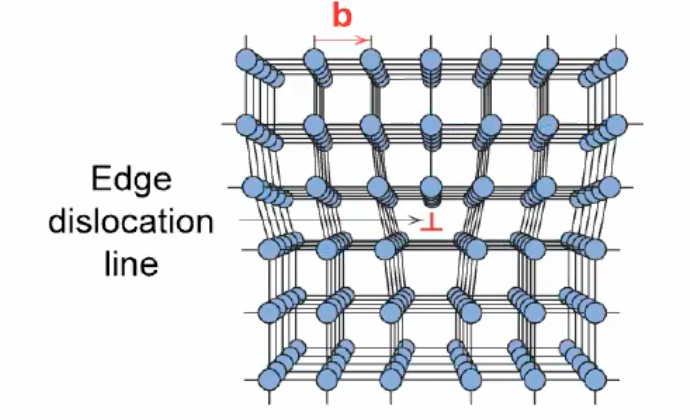
\includegraphics[width=\textwidth]{images/Edge.png}
    \end{figure}
    \textbf{Screw Dislocations}
    \begin{enumerate}
        \item spiral planar ramp resulting from shear deformation
        \item b is parallel $\parallel$ to dislocation line
    \end{enumerate}
    \begin{figure}[H]
        \centering
        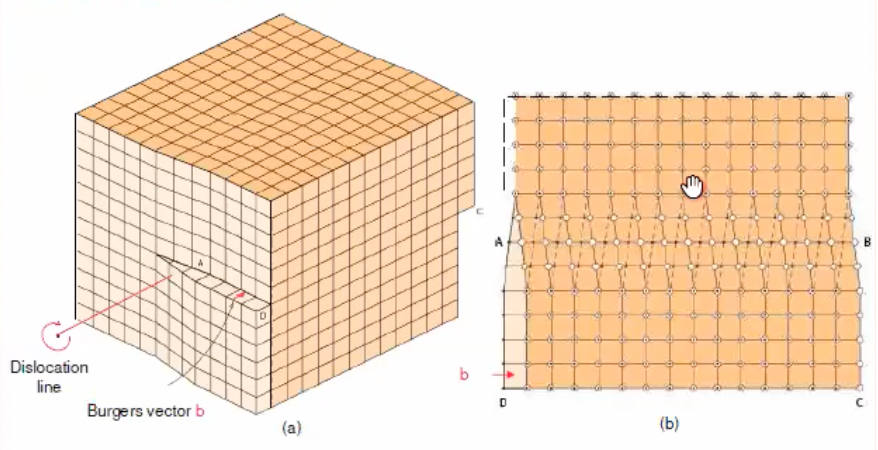
\includegraphics[width=\textwidth]{images/Screw.png}
    \end{figure}
    \textbf{Twin boundary (plane)}
    \begin{enumerate}
        \item Relfection of atom positions across the twin plane
    \end{enumerate}
    \begin{figure}[H]
        \centering
        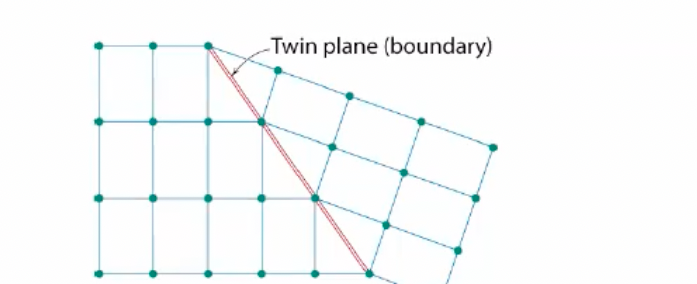
\includegraphics[width=\textwidth]{images/Twin.png}
    \end{figure}
    \textbf{Staking Faults}
    \begin{enumerate}
        \item For FCC – An error in ABc packing sequence
        \item e.g. ABCABCABC $\rightarrow$ ABCABABC
    \end{enumerate}
    \pagebreak
    \subsection{Diffusion}
    \textbf{Inter-Diffusion:} 
    In an alloy, atoms migrate from regions of high 
    concentration to regions of low concentration \\
    \textbf{Self-Diffusion:} 
    In an elemental solid, atoms migrate \\
    \textbf{Vacancy Diffusion:}
    Atoms exchange vacancies. The rate depends on the concentration
    of vacancies and the activation energy for an exchange \\
    \textbf{Intersitial Diffusion:}
    Smaller atoms diffuse between host attoms. This happens more rapidly than vacancy
    diffusion because they aren't strongly 
    \subsubsection{Time independant}
    \begin{flalign}
        &J = \frac{M}{At} = \frac{1}{A}\frac{dM}{dt}& \\
        &J = -D\frac{dC}{dx} \\
        & \text{If linear } \frac{dC}{dx} \cong \frac{\Delta C}{\Delta x} = \frac{C_2 - C_1}{x_2-x_2} \\
        & D = D_0\cdot e^{-\frac{Q_d}{RT}} \\
    \end{flalign}
    \subsubsection{Non Steady State Diffusion}
    \begin{flalign}
        & \frac{\partial C}{\partial t} = D\frac{\partial^2 C}{\partial x^2} & \\
        &\frac{C(x,t) - C_0}{C_s - C_0} = 1 - erf\left(\frac{x}{2\sqrt{Dt}}\right),
        \;\text{where: } erf(z)=\frac{2}{\sqrt{\pi}} \int_0^ze^{-y^2}dy
    \end{flalign}
    \pagebreak
    \section{Phase diagrams}
    \textbf{Lever Rule}
    \begin{flalign}
       & M_\alpha\times S = M_L\times R &\\
        &W_L = \frac{M_L}{M_L + M_\alpha} = \frac{S}{R+S} = \frac{C_\alpha - C_0}{C_\alpha - C_L} \\
        &W_\alpha = \frac{R}{R + S} = \frac{C_0 - C_L}{C_\alpha - C_L}
    \end{flalign}
    \begin{figure}[H]
        \centering
        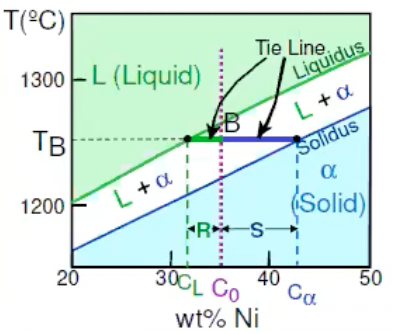
\includegraphics[width=\textwidth]{images/Lever.png}
    \end{figure}
\end{document}